\documentclass[xcolor=table]{beamer}
\usepackage{fontspec}
\usepackage{natbib}
\usepackage{gb4e} 
\usepackage[table]{xcolor}
\usepackage{booktabs} 
%\usepackage{color}
\usepackage{graphicx}
\usepackage{bibentry}
\usepackage{tikz}
\usetikzlibrary{trees}

% \setmainfont[Mapping=tex-text]{Charis SIL}
\let\sfdefault\rmdefault
%\newcommand{\racine}[1]{\begin{math}\sqrt{#1}\end{math}} 
\newfontfamily\phon[Mapping=tex-text,Ligatures=Common,Scale=MatchLowercase,FakeSlant=0.3]{Charis SIL} 
\newcommand{\ipa}[1]{{\phon \mbox{#1}}} %API tjs en italique
\newcommand{\grise}[1]{\cellcolor{lightgray}\textbf{#1}} 
\newcommand{\ra}{$\Sigma_1$} 
\newcommand{\rc}{$\Sigma_3$} 
\newcommand{\ro}{$\Sigma$} 
 \begin{document}

 \title{Linguistique panchronique: terrain, formalisation et implémentation}
 \author{Guillaume Jacques}
 \date{}
 \maketitle


 \begin{frame} 
 \frametitle{Publications additionnelles}
 \bibliographystyle{unified}
   \nobibliography{bibliogj.bib}
   
\begin{itemize}
\item  \bibentry{jacques14ergative}  
\item  \bibentry{jacques15causative}
\item  \bibentry{jacques15spontaneous}
\item  \bibentry{jacques15derivational.khaling}
\end{itemize}
 \end{frame}
 
  \begin{frame} 
 \frametitle{Projet de recherche} 
 \begin{figure}[H]
\centering
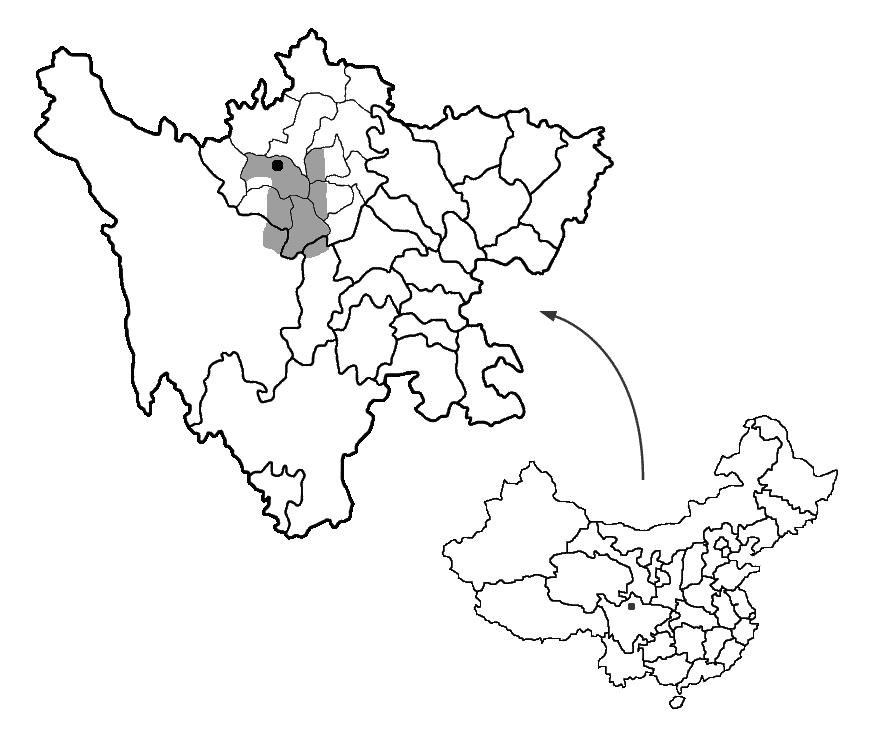
\includegraphics[height=28mm]{carte.JPG}
\end{figure}

\begin{itemize}[<+->]
\item Grammaire Japhug
\item Linguistique comparative des langues rgyalronguiques et kiranties.
\item Phonologie panchronique
\item Morphosyntaxe panchronique (systèmes d'indexation, l'origine des marques de voix, la typologie des langues OV préfixantes et l'évidentialité nominale)
\item Modélisation formelle de la méthode comparative 
\end{itemize}
   
  \end{frame}   


  \begin{frame} 
 \frametitle{Approche collaborative de la recherche} 
 \framesubtitle{Doctorants} 

\begin{enumerate}
\item Gong Xun (Zbu)
\item Lai Yunfan (Khroskyabs)
\item Gao Yang (Menya)
\item Rao Min (Guiqiong)
\end{enumerate}

\begin{itemize}
\item  \bibentry{lai13fuyin}
\item  \bibentry{gongxun14agreement}  
\item  \bibentry{lai14person}
\end{itemize}   
  \end{frame}   

\end{document}